% 2006 湖南文科第10题：向量系数可行域
% 阴影为射线 OM、线段 OB 与 AB 延长线围成的无界带在图中截取的代表性有限部分；
% 上边界 L--T 只由灰色填充表示，原图不描边。
\usetikzlibrary{arrows.meta}
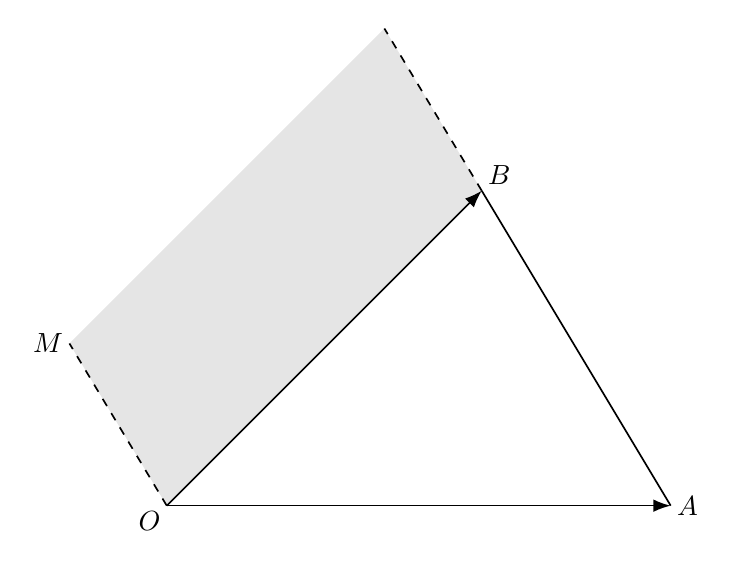
\begin{tikzpicture}[x=1cm,y=1cm,line width=.6pt,font=\normalsize]
\coordinate (O) at (0,0);
\coordinate (A) at (6.4,0);
\coordinate (B) at (4,4);
\coordinate (L) at (-1.236,2.06);
\coordinate (T) at (2.764,6.06);
\fill[black!10] (O)--(L)--(T)--(B)--cycle;
\draw[-{Latex[length=2.2mm,width=1.6mm]}] (O)--(A);
\draw[-{Latex[length=2.2mm,width=1.6mm]}] (O)--(B);
\draw (A)--(B);
\draw[dashed] (O)--(L);
\draw[dashed] (B)--(T);
\node[below left,inner sep=2pt] at (O) {$O$};
\node[right,inner sep=2pt] at (A) {$A$};
\node[above right,inner sep=2pt] at (B) {$B$};
\node[left,inner sep=2pt] at (L) {$M$};
\end{tikzpicture}
